\documentclass[12pt, a4paper, table]{article}
%\usepackage[utf8]{inputenc}
\usepackage[T1]{fontenc}
\usepackage[francais]{babel}
\usepackage{textcomp}
\usepackage{mathtools,amssymb,amsthm}
\usepackage[left = 2cm, top = 1.33cm, right = 2cm, bottom = 2.3 cm, headheight = 0pt]{geometry}
\usepackage{graphicx}
\usepackage{pgf, tikz}
	\usetikzlibrary{arrows,shapes,positioning}
\usepackage{centernot}
\usepackage{pgffor, ifthen}
\usepackage{lmodern}
\usepackage{colortbl}
\usepackage{array}
\usepackage{calc}
\usepackage{titlesec}
\usepackage{titletoc}
\usepackage{fancyhdr}
\usepackage{fancybox}
\usepackage{titling}
\usepackage{enumitem}
\usepackage{wrapfig}
\usepackage{caption}
\usepackage{tocloft}
\usepackage{epigraph}
\usepackage{lipsum}
\usepackage{ulem}
\usepackage{multirow}
\usepackage{hhline}
\usepackage{xcolor}
\usepackage{listings}
\usepackage{hyperref}
\definecolor{light-gray}{gray}{0.95}
\setcounter{tocdepth}{0}

\titleformat{\section}
  {\normalfont\sffamily\Large\bfseries}
  {\thesection.}{0.5em}{}

\titleformat{\subsection}
  {\normalfont\sffamily\large\bfseries}
  {\thesubsection}{0.5em}{}
\titleformat{\subsubsection}
  {\normalfont\sffamily\normalsize\bfseries}
  {}{0.5em}{}


\definecolor{pblue}{rgb}{0.13,0.13,1}
\definecolor{pgreen}{rgb}{0,0.5,0}
\definecolor{pred}{rgb}{0.9,0,0}
\definecolor{pgrey}{rgb}{0.46,0.45,0.48}


\lstset{language=Java,
 basicstyle=\footnotesize\tt,
  showspaces=false,
  showtabs=false,
  breaklines=true,
  showstringspaces=false,
  breakatwhitespace=true,
  commentstyle=\color{pgreen},
  keywordstyle=\color{pblue},
  stringstyle=\color{pred},
  moredelim=[il][\textcolor{pgrey}]{},
  moredelim=[is][\textcolor{pgrey}]{\%\%}{\%\%},
    numbers=left,
    numberstyle=\color{pgrey}, % the style that is used for the line-numbers
  rulecolor=\color{black}
}

\pagestyle{fancy}

\setlength{\headheight}{15pt} 

\renewcommand{\headrulewidth}{1pt}
\fancyhead[C]{} 
\fancyhead[L]{\textsf{Groupe 14 \\ Antoine Duchêne - Justin Michaux}}
\fancyhead[R]{\textsf{LSINF1103 \\ Introduction à l'algorithmique}}

\renewcommand{\footrulewidth}{1pt}
\fancyfoot[C]{}
\fancyfoot[R]{\textbf{\textsf{\thepage}}}
\fancyfoot[L]{\textbf{\textsf{\today}}}

\begin{document}


\begin{Large} \begin{center}
\vspace{-0.83cm}
\noindent \rule{15cm}{.9pt} 
\vspace{-0.33cm}
	\textsf{Mini-projet 2 -  Conception d’algorithme : Troycount}\\
	\rule{15cm}{.9pt} 
\end{center} \end{Large} 
\vspace{-0.7cm}
\section{Explication de l'algorithme}
\vspace{-0.3cm}
\subsection{Procédure}
\begin{enumerate}
\item Créer un tableau de personne (Voir figure 2)
\item Ordonner ce tableau en fonction de la balance financière de chaque personne
\item Séparer le tableau en 2
\begin{itemize}
\item Personnes ayant une balance positive (= débiteurs)
\item Personnes ayant une balance négative (= créanciers) \medskip \\
NB: Les personnes ayant une balance nulle sont enlevées (Elle ne doivent pas \\ donner/recevoir d'argent)
\end{itemize}
\item Parcourir le tableau de débiteurs et de créanciers
\item A chaque itération, effectuer les transactions appropriées (Voir 1.2 gestion des transactions)
\end{enumerate}

\noindent \begin{minipage}{0.5 \textwidth}
\begin{center}
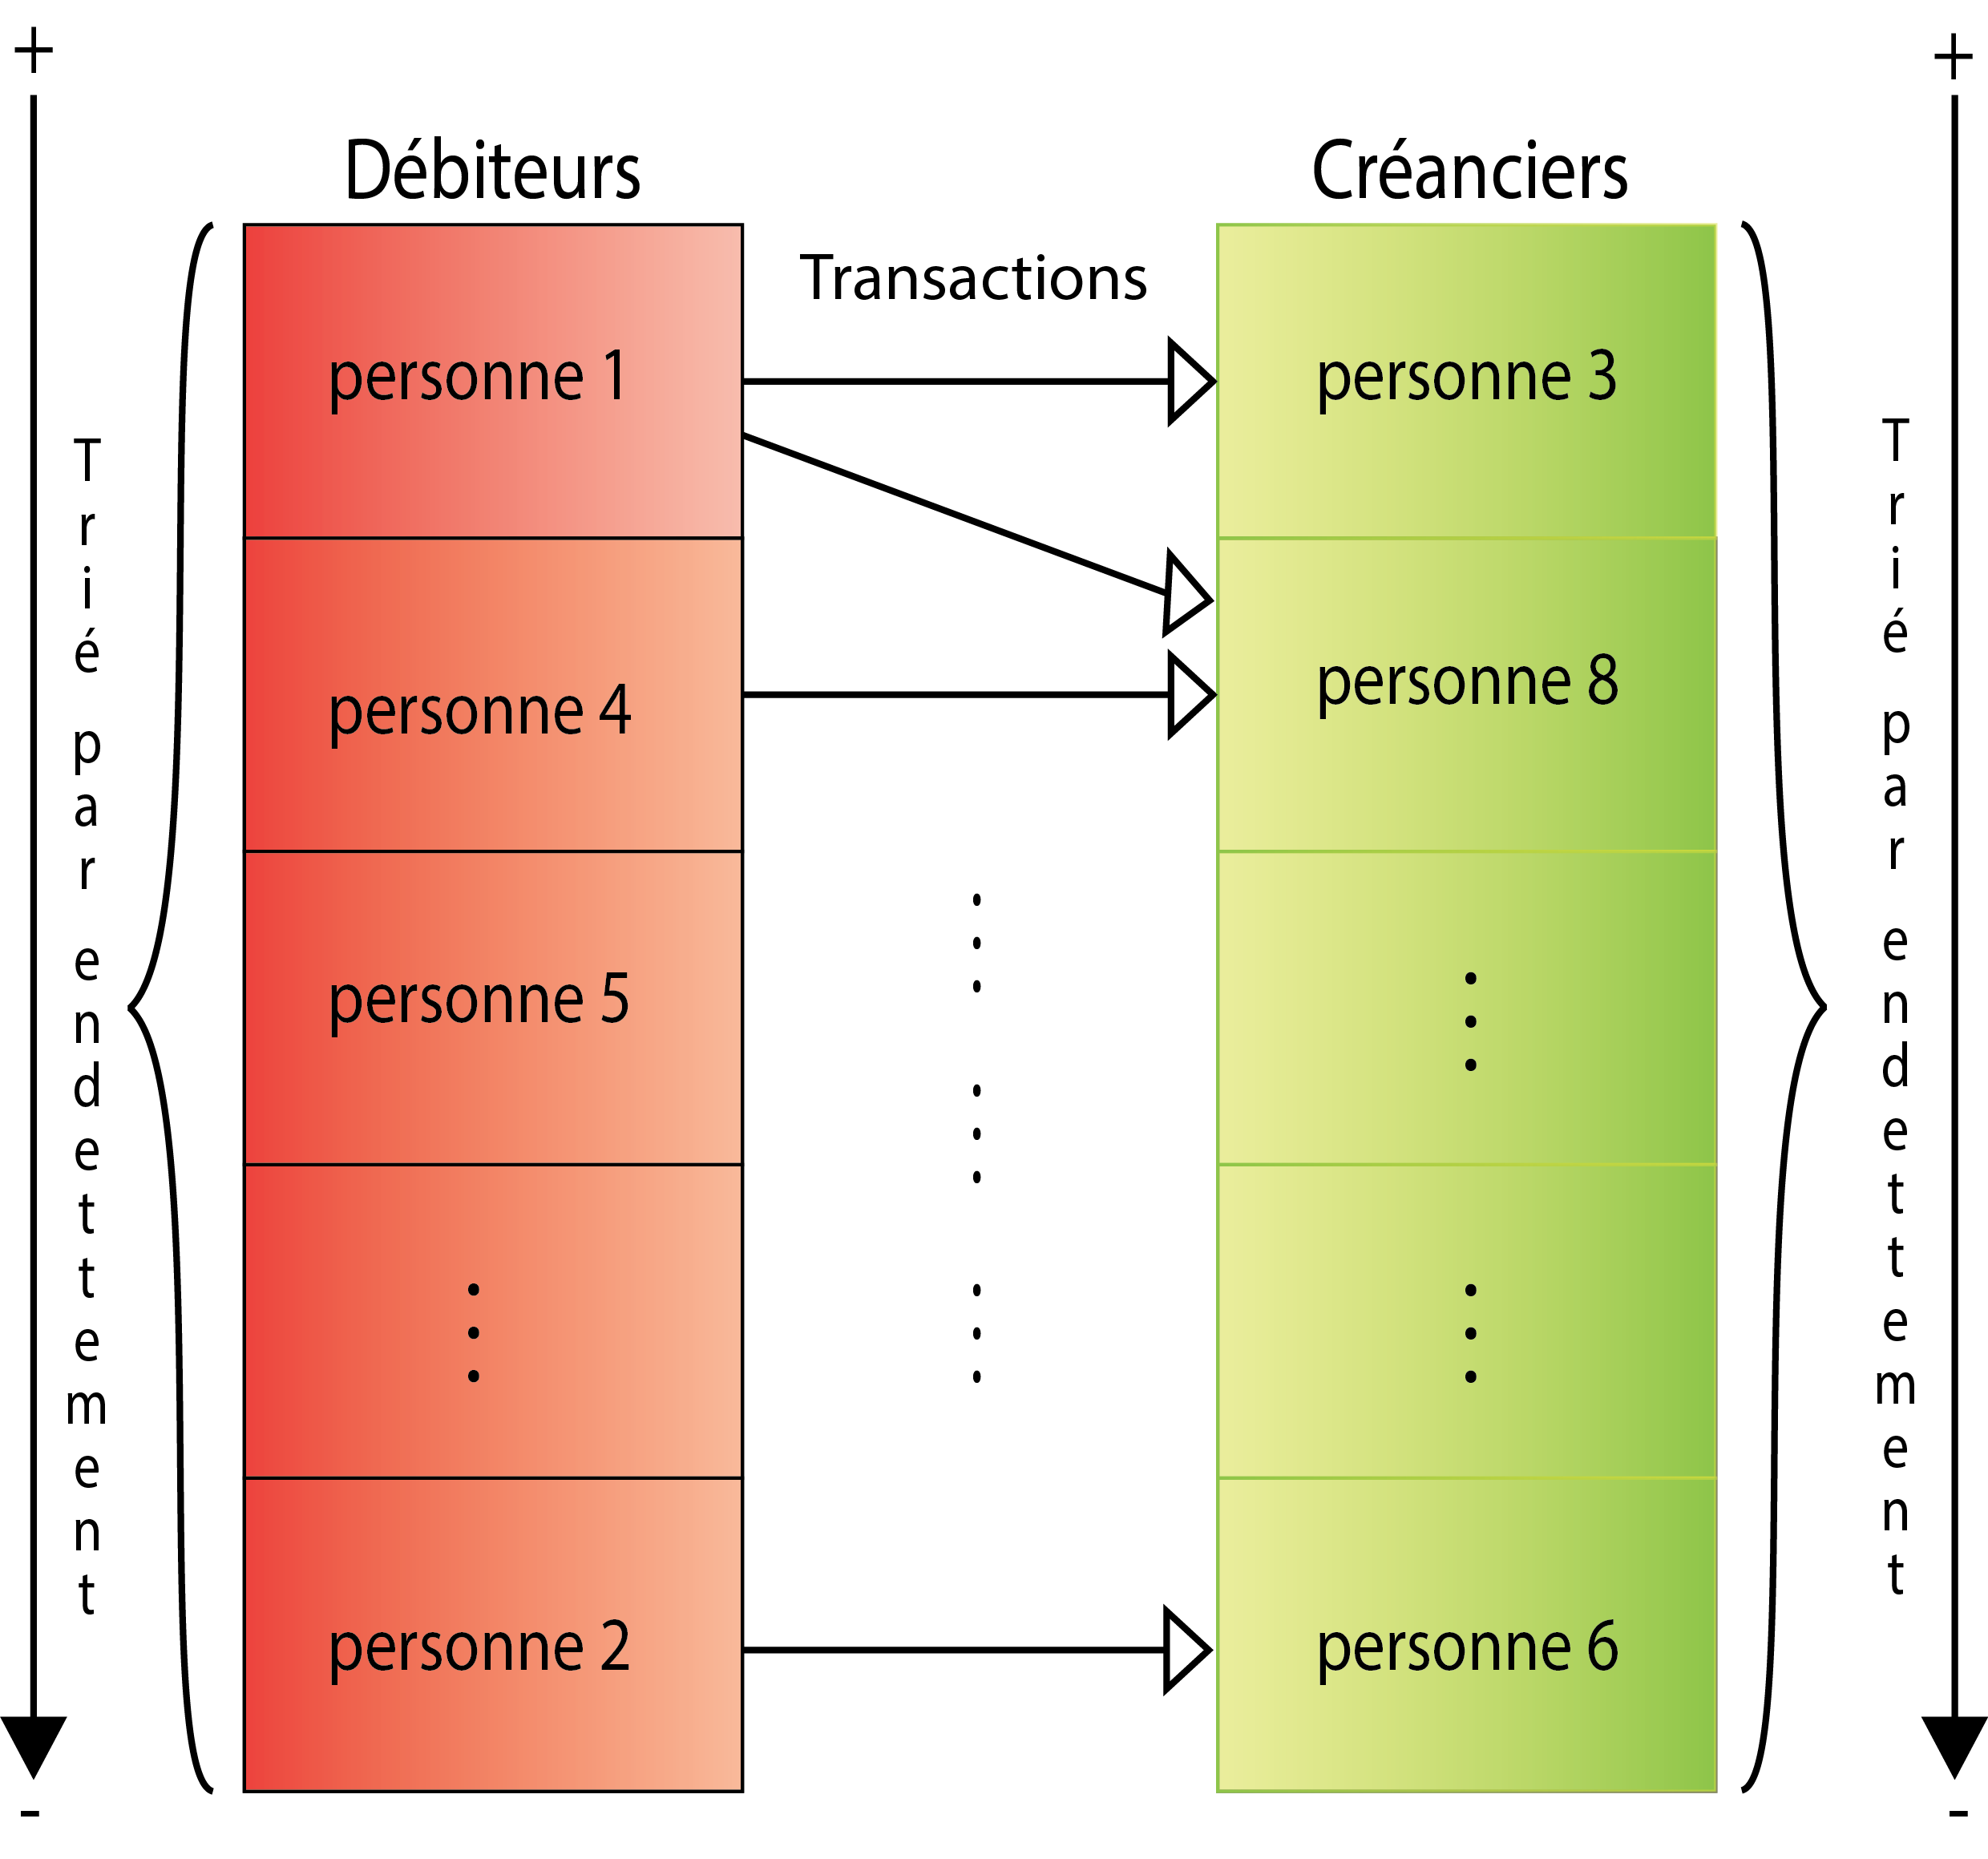
\includegraphics[scale=0.33]{sch}
\captionof{figure}{Création des transactions}
\label{image-tigre}
\end{center}
\end{minipage}
\begin{minipage}{0.5 \textwidth}
\begin{center}
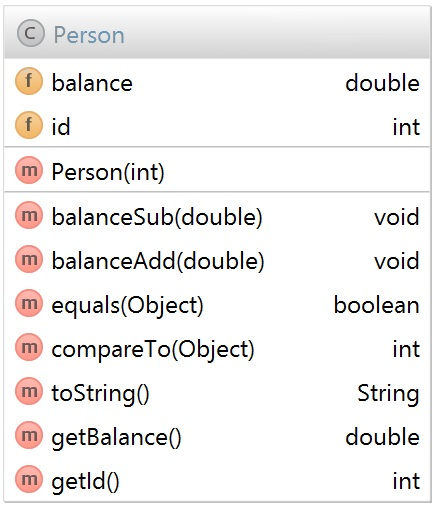
\includegraphics[scale=0.33]{per2}
\captionof{figure}{Objet "personne"}
\label{image-tigre}
\end{center}
\end{minipage}
\subsection{Gestion des transactions}
\noindent Afin de gérer les transactions, les 2 tableaux sont parcourus simultanément (personnes créancières et personnes débitrices) 
\smallskip \\
\noindent \textbf{Fonctionnement}

\begin{enumerate}
\item Commencer au début de chaque tableau
\item Comparer le débiteur actuel avec le créancier actuel; 2 situations :
\begin{enumerate}
\item le débiteur actuel peut rembourser intégralement le créancier actuel
\begin{enumerate}
\item Le débiteur lui verse toute la créance
\item Passer au créancier suivant 
\end{enumerate} 
\item le débiteur ne peut rembourser intégralement le créancier actuel
\begin{enumerate}
\item Le débiteur lui verse toute sa dette
\item Passer au débiteur suivant 
\end{enumerate} 
\end{enumerate}
\item Recommencer l'étape 2 jusqu'à la fin des tableaux
\end{enumerate}
 \footnotesize{NB: Les transactions sont stockées au fur et à mesure dans une pile. Celle-ci et ensuite retournée sous forme d'un tableau }








\vspace{-6pt}
\section{Complexité des différentes méthodes}
\normalsize
\noindent Soit n, le nombre de personnes : n représente donc la taille du problème à résoudre.
\vspace{-6pt}
\subsection{Troycount.balance()}
\noindent Complexité temporelle en $\mathbf{\Theta (n)}$ car :

\begin{enumerate}
	\item L'expression sera toujours parcourue entièrement 1 fois, à l'aide d'une boucle.
	\item La boucle principale ne contient que des opérations de complexité $\mathbf{\Theta (1)}$.
\end{enumerate}

\noindent On en déduit donc que le temps d'exécution augmentera de façon linéaire par rapport à la taille du problème.

\subsection{Troycount.generateTabPerson}
\noindent Complexité temporelle en $\mathbf{\mathcal{O}(}\mathbf{log (n))}$ car :
\begin{enumerate}
	\item Complexité temporelle en $\mathbf{\mathcal{O}(h)}$, où h est la hauteur de l’arbre
	\item L'arbre est équilibré donc h $\in$ $\mathbf{\Theta(\mathbf{log}_{2} (n))}$
\end{enumerate}
Donc, 
\begin{itemize}
	\item Meilleur cas : $\mathbf{\Theta (1)}$ (on tombe sur la racine)
	\item Pire cas : $\mathbf{\Theta(}\mathbf{log (n))}$
	\item En général : $\mathbf{\mathcal{O}(}\mathbf{log (n))}$
\end{itemize}



\section{Choix d'implémentation}

Afin d'implémenter notre algorithme nous avons utilisé la programmation orienté objet; Une classe "personne" a été créer afin de gérer plus facilement les créances et dettes de chaque personne. De plus, cette classe "personne" implémente l'interface "Comparable" ce qui permet de trier facilement les créanciers et les débiteurs. 



\newpage
\section*{Annexe}

\subsection*{Troycount.balance()}

\begin{lstlisting}[language=Java]
public Transaction[] balance() {
    Person[] persons = generateTabPersons();
    Arrays.sort(persons);

    int firstSplitIndex = 0;
    int secondSplitIndex = 0;

    for (int i = 0; persons[i].getBalance() >= 0; i++) {
    	secondSplitIndex++;
    	if (persons[i].getBalance() > 0) {
    		firstSplitIndex++;
        }
     }

    Person[] debtors = Arrays.copyOfRange(persons, 0, firstSplitIndex);
    Person[] creditors = Arrays.copyOfRange(persons, secondSplitIndex, persons.length);

    reverse(creditors);

    Stack<Transaction> transactions = new Stack<Transaction>();
    int i = 0, j = 0;

    while (i < debtors.length && j < creditors.length) {
        if (debtors[i].getBalance() <= -creditors[j].getBalance()){
            double transactionAmount = debtors[i].getBalance();
            Transaction t = new Transaction(debtors[i].getId(),
                                            creditors[j].getId(),
                                            transactionAmount);
            transactions.add(t);
            System.out.println(t);
            creditors[j].balanceAdd(transactionAmount);
            debtors[i].balanceSub(transactionAmount);
            i++;
        } else {
            double transactionAmount = -creditors[j].getBalance();
            Transaction t = new Transaction(debtors[i].getId(),
                                            creditors[j].getId(),
                                            transactionAmount);
            transactions.add(t);
            System.out.println(t);
            creditors[j].balanceAdd(transactionAmount);
            debtors[j].balanceSub(transactionAmount);
            j++;
		}
	}
    return transactions.toArray(new Transaction[transactions.size()]);
}
\end{lstlisting}
\newpage
\subsection*{Troycount.generateTabPerson()}
\begin{lstlisting}
public Person[] generateTabPersons() {
   Person[] persons = new Person[group_size];
   for (int i = 0; i < group_size; i++) {
      int personID = i + 1;
      persons[i] = new Person(personID);
   }
   for (Spending aSpending : spendings) {
      int debitedPerson = aSpending.get_paid_by()
      int[] chargedPerson = aSpending.get_paid_for();
      int chargedPersons = chargedPerson.length;
      double spendingAmount = aSpending.get_amount();
  
      for (int person : chargedPerson) { 
         double fixedCharge = aSpending.get_fixed_charges(person);
         spendingAmount -= fixedCharge;
      } 
      
      for (int person : chargedPerson) {
         persons[person - 1].balanceAdd(spendingAmount / chargedPersons);
      }
  
      persons[debitedPerson - 1].balanceSub(spendingAmount);
  }
  return persons;
}
\end{lstlisting}







\end{document}